\section{Technical Approach}
\label{sec:TechnicalApproach}

\begin{figure}
\centering
\begin{subfigure}[b]{0.69\textwidth}
        \centering
        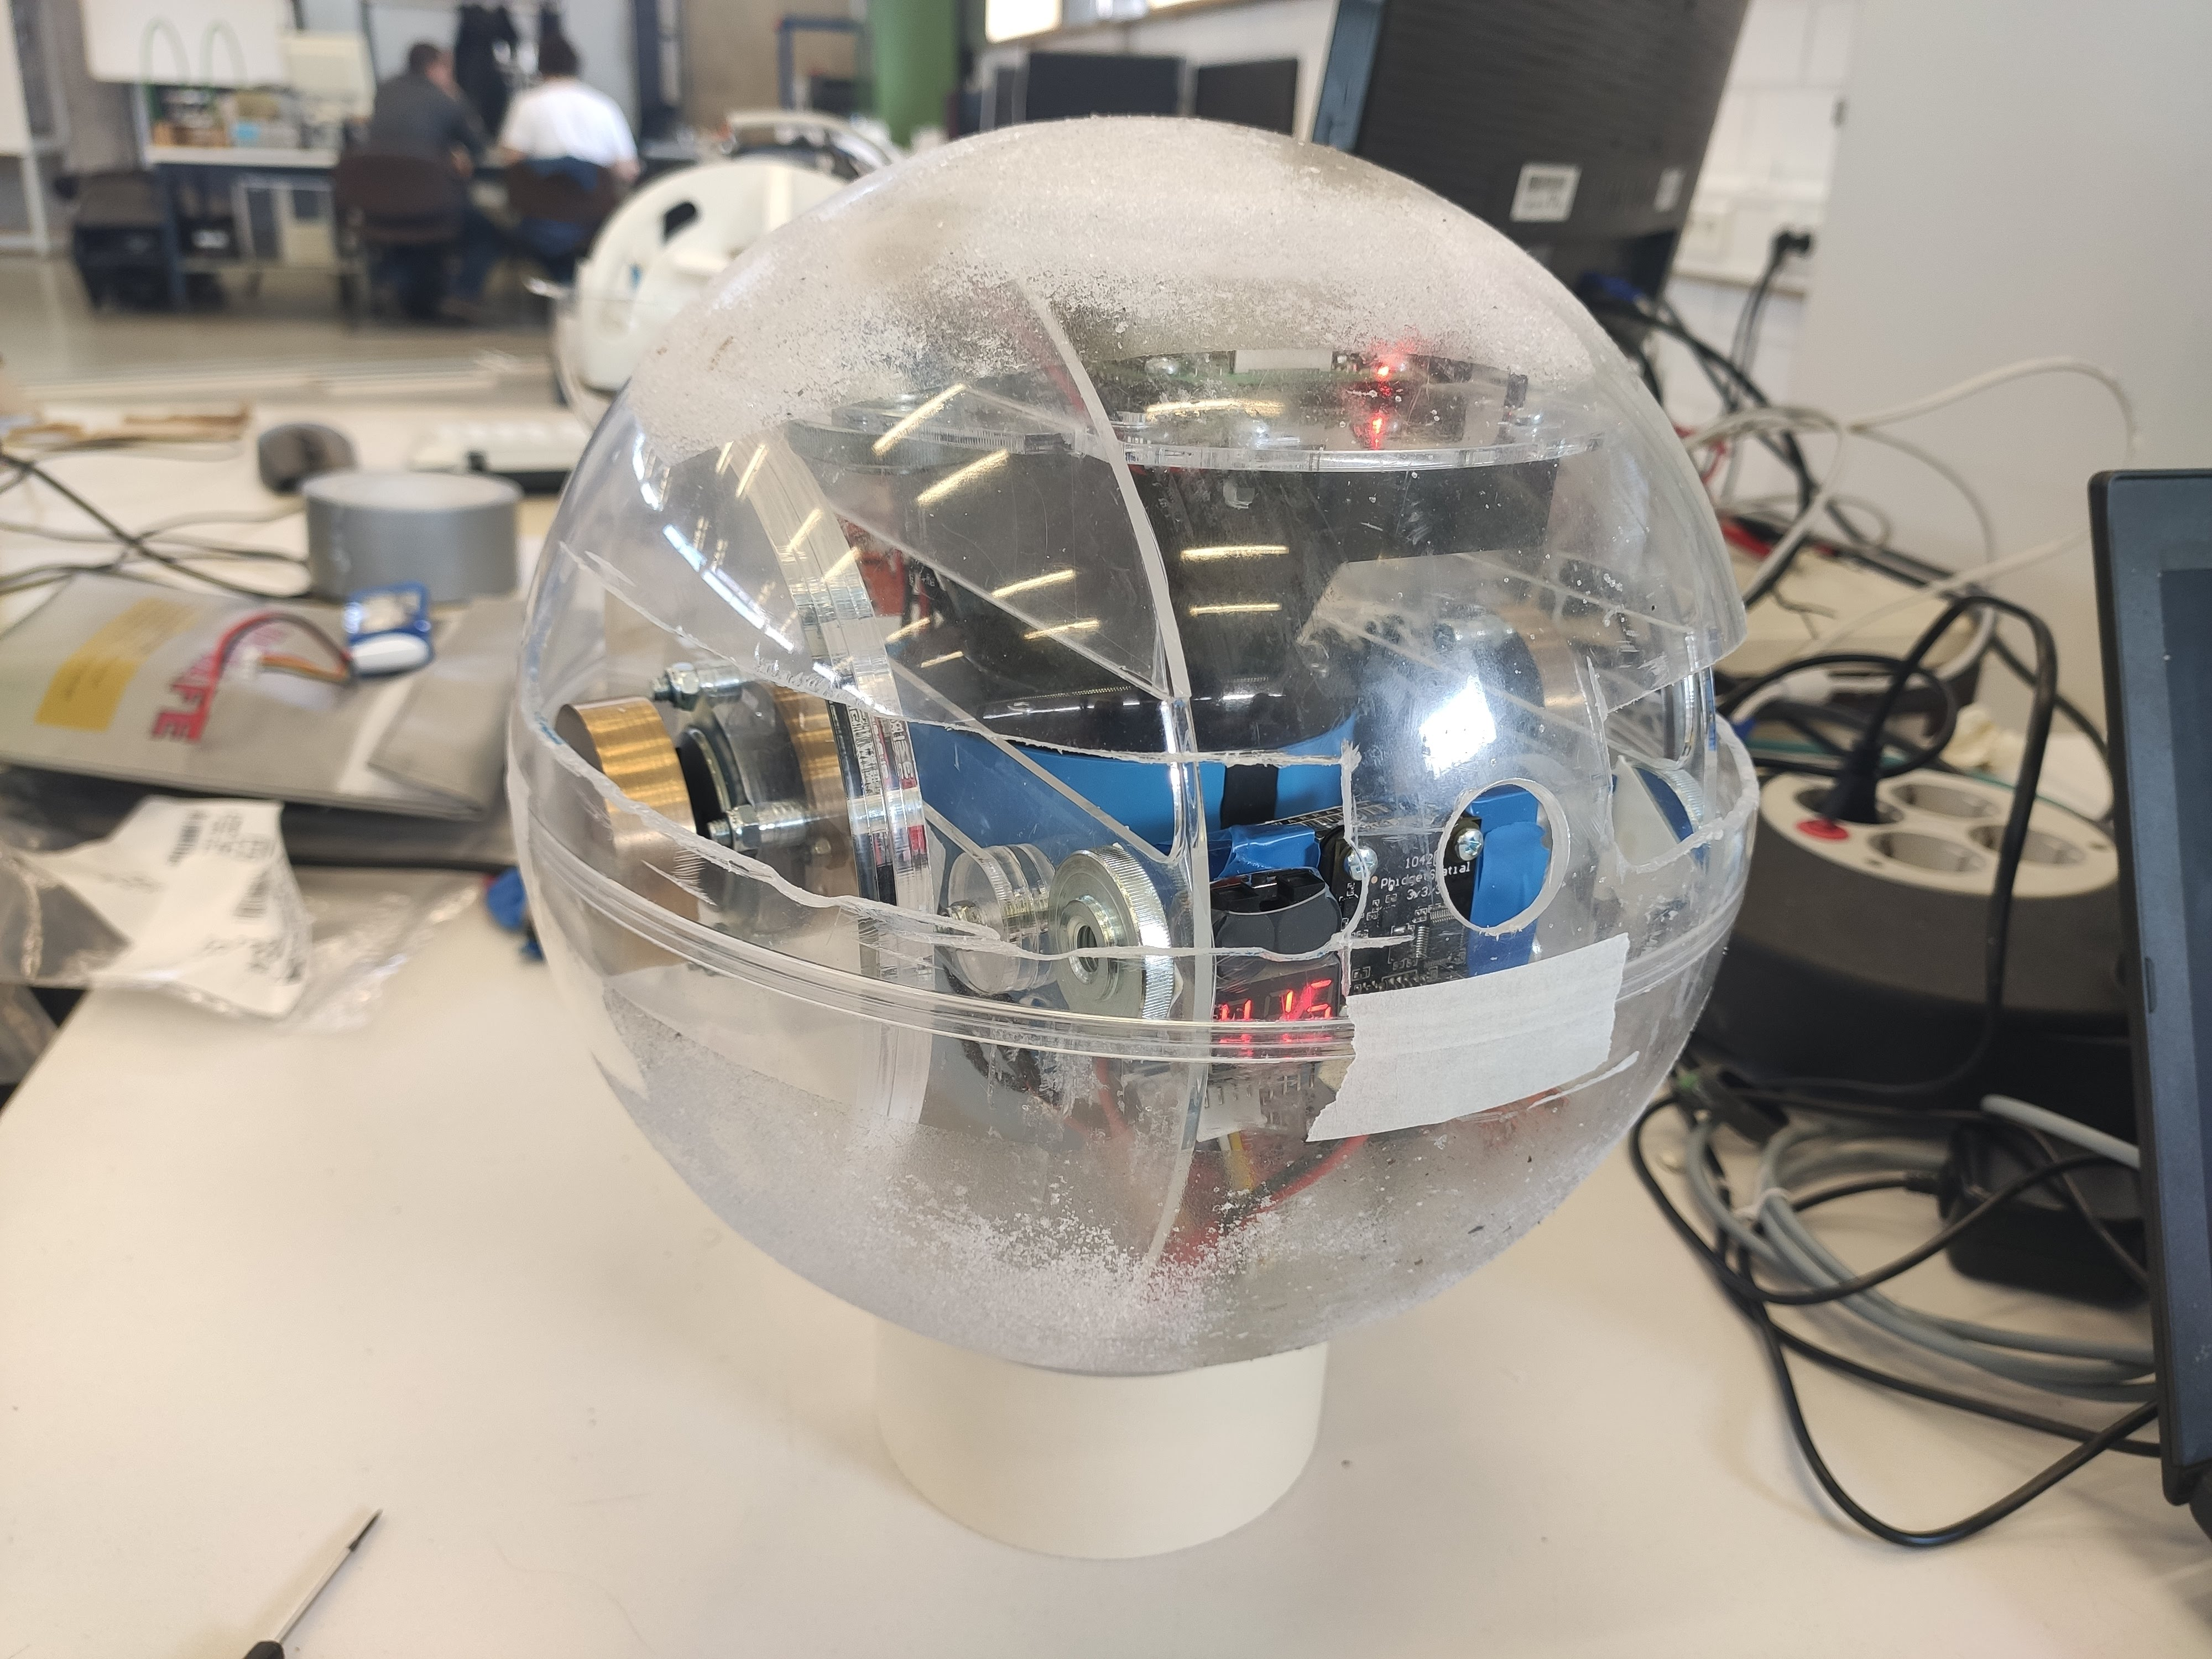
\includegraphics[width=\textwidth]{../Media/sphereFullshellLeft.jpg}
        \caption{Hardware setup of the L.U.N.A sphere prototype, including notches in the shell and friction granule.}
        \label{sec:TechnicalApproach:fig:prototype}
\end{subfigure}
\hfill
\begin{subfigure}[b]{0.3\textwidth}
        \centering
        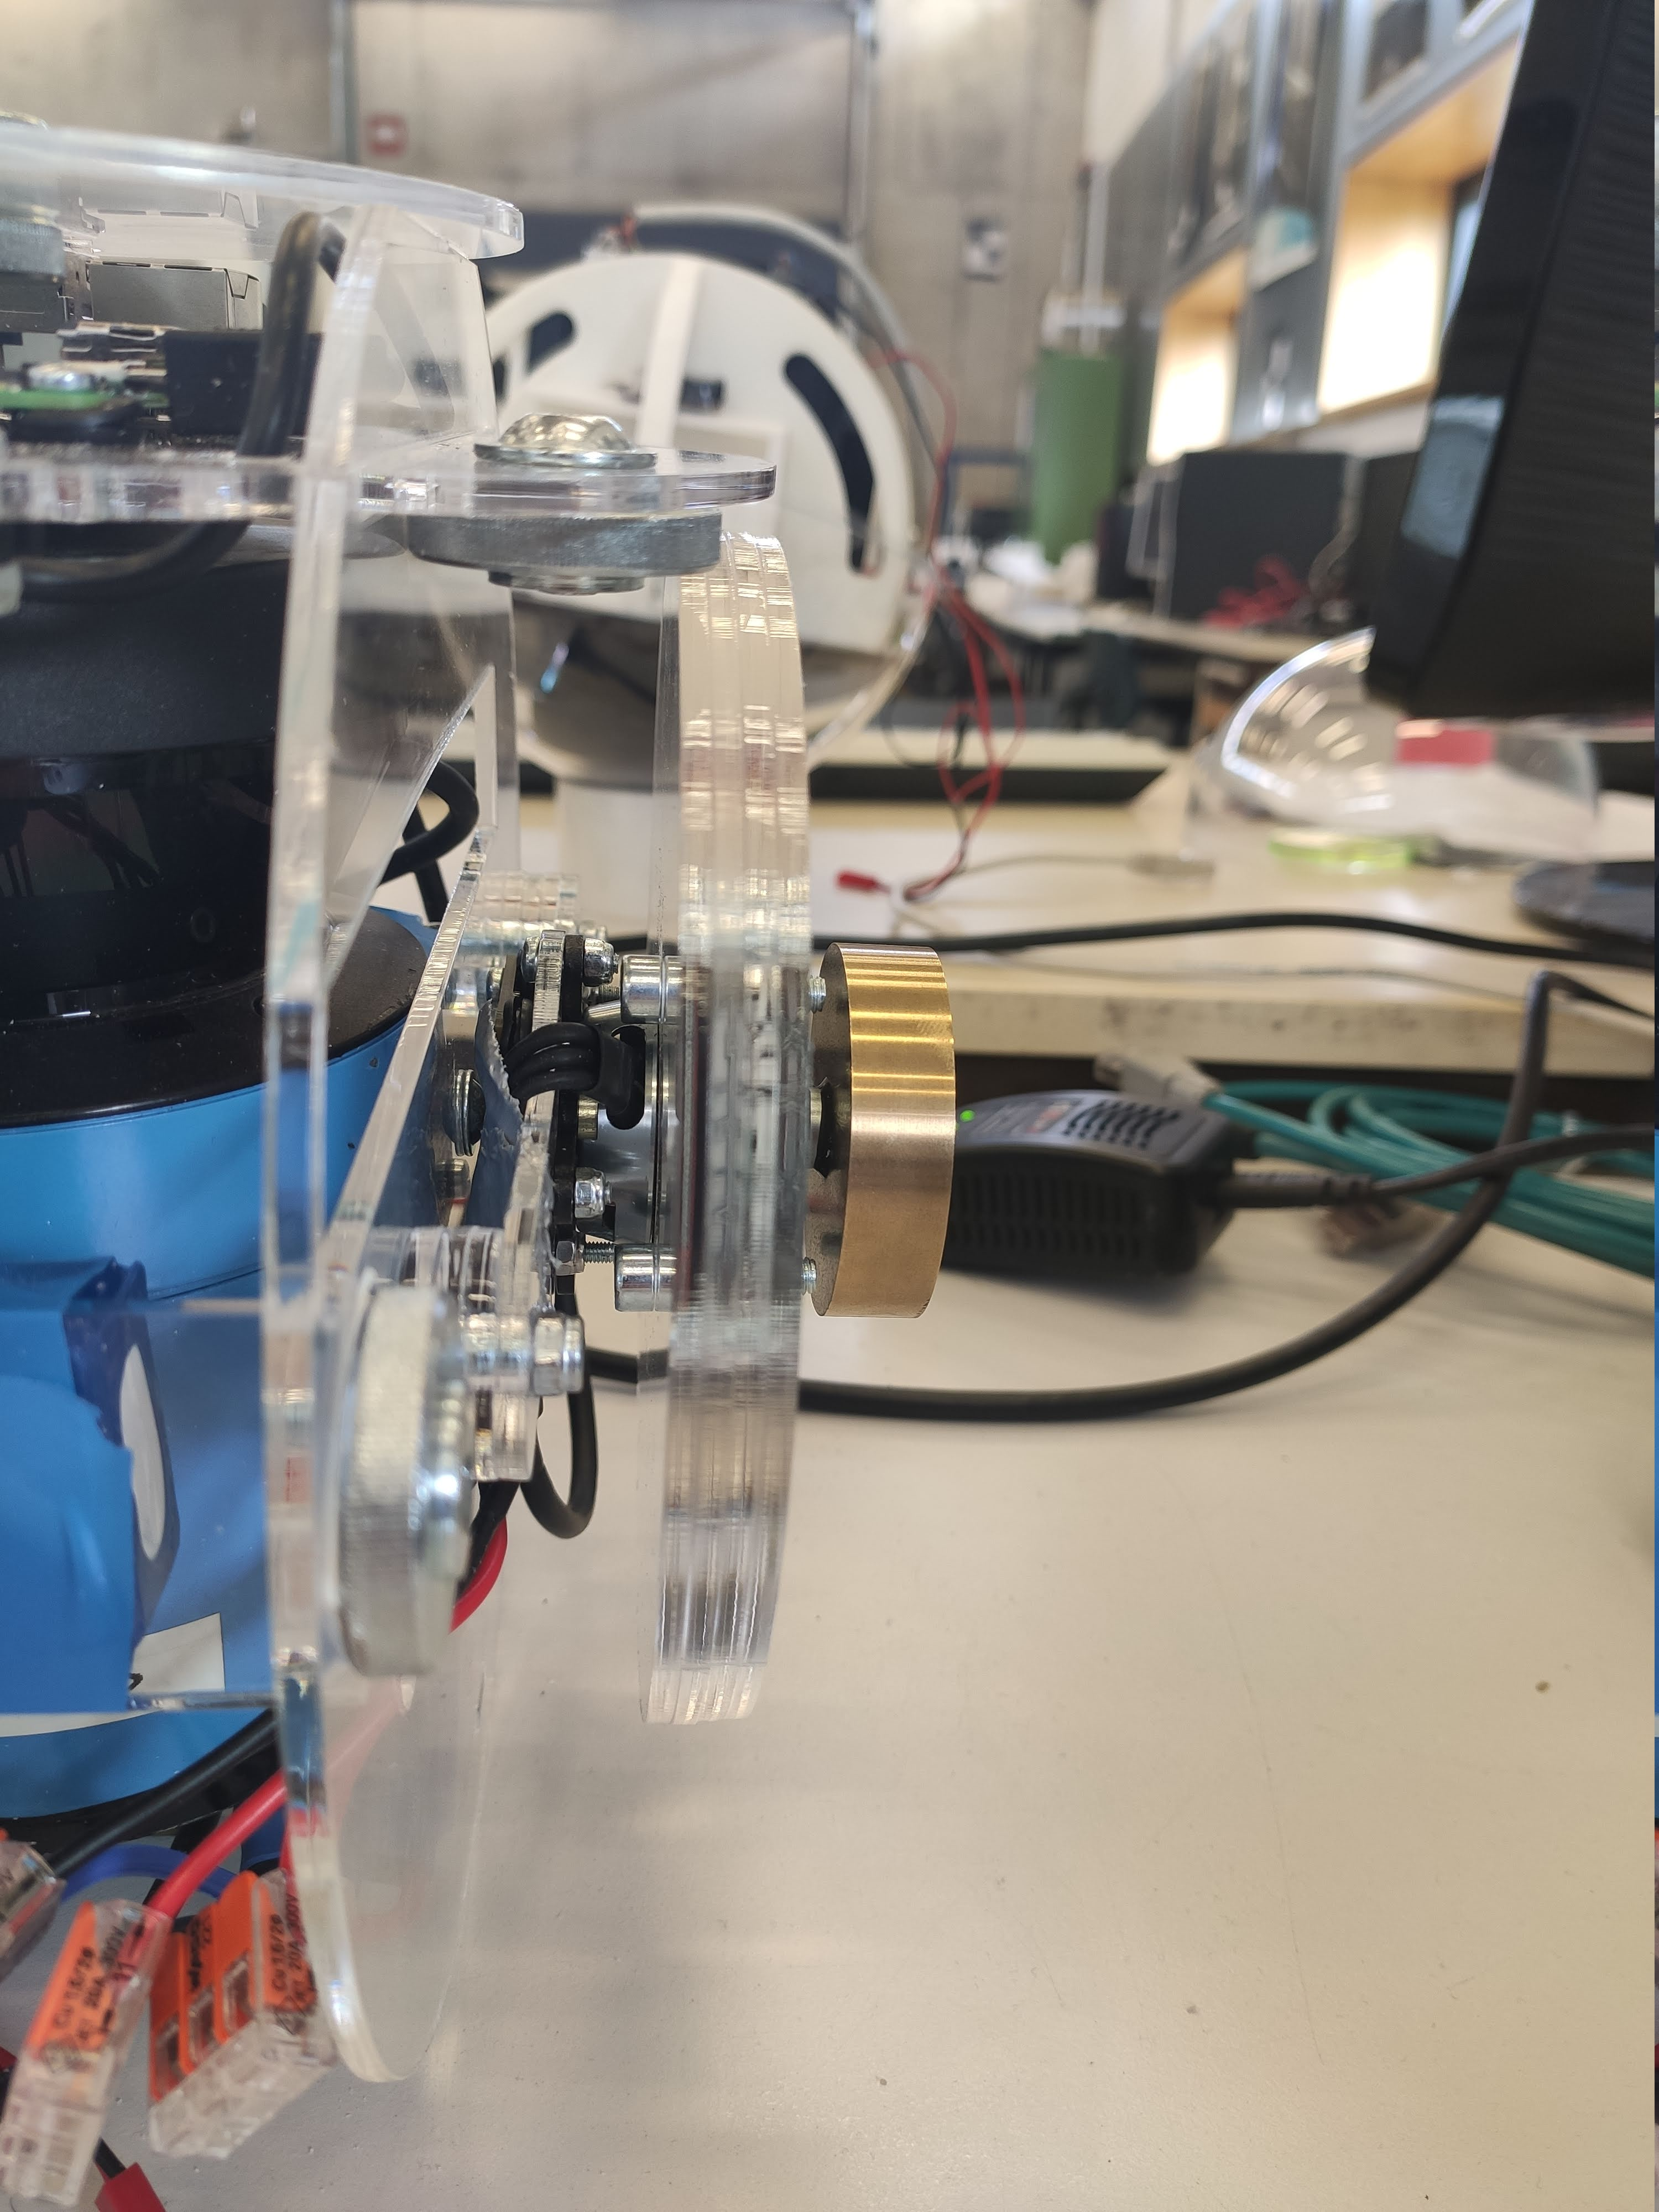
\includegraphics[width=\textwidth]{../Media/sphereRightMotor.jpg}
        \caption{IMU (beneath supporting structure) and brushless motor (above supporting structure) of the L.U.N.A sphere without shell, including flywheel mass. }
        \label{sec:TechnicalApproach:fig:motor}
\end{subfigure}
\caption{Hardware setup of the L.U.N.A sphere prototype, including notches in the shell and friction granule.}
\end{figure}

Figure \ref{sec:TechnicalApproach:fig:prototype} shows the final hardware setup of the robot. In order to reduce complexity with respect to the 3D-transformation calculations, the laserscanner was placed at the center of a spherical acrylic glass shell as precisely as possible. This limits the laser scanners movement to rotational movement and removes translational movement completely. With this initial setup given, the only room left for the acrylic glass structural components, batteries, boardcomputer, IMUs, motors, weights and wiring are the spaces between the scanner and the shell. Figure \ref{sec:TechnicalApproach:fig:motor} shows one Turnigy Park480 brushless outrunner motor \cite{turnigymotor} of the COAM drive with two flywheels attached. Strong epoxy glue attaches the weights to the motor shafts and shells. As the flywheels start spinning with respect to the structural components of the sphere, the sphere itself starts spinning with respect to the ground. 

\subsection{Hardware Setup}
\label{sec:TechnicalApproach:HardwareSetup}

Figure \ref{sec:TechnicalApproach:fig:prototype} also shows that the top and the bottom of the shell are covered in table salt, which made a good granule to increase friction to the ground in the early testing phase. Furthermore, there are notches in the front side of the shell to increase permeability for the laser. Unfortunately, the laser scanner measurements are still very much affected by blockades due to components of the sphere. Specifically, the outside shell is a strongly inhibiting factor as an object with the distance of the radius is measured at all times.
                                                                                                                                                                                                                  
\begin{figure}                                                                                                                                                                                                    
\centering                                                                                                                                                                                                        
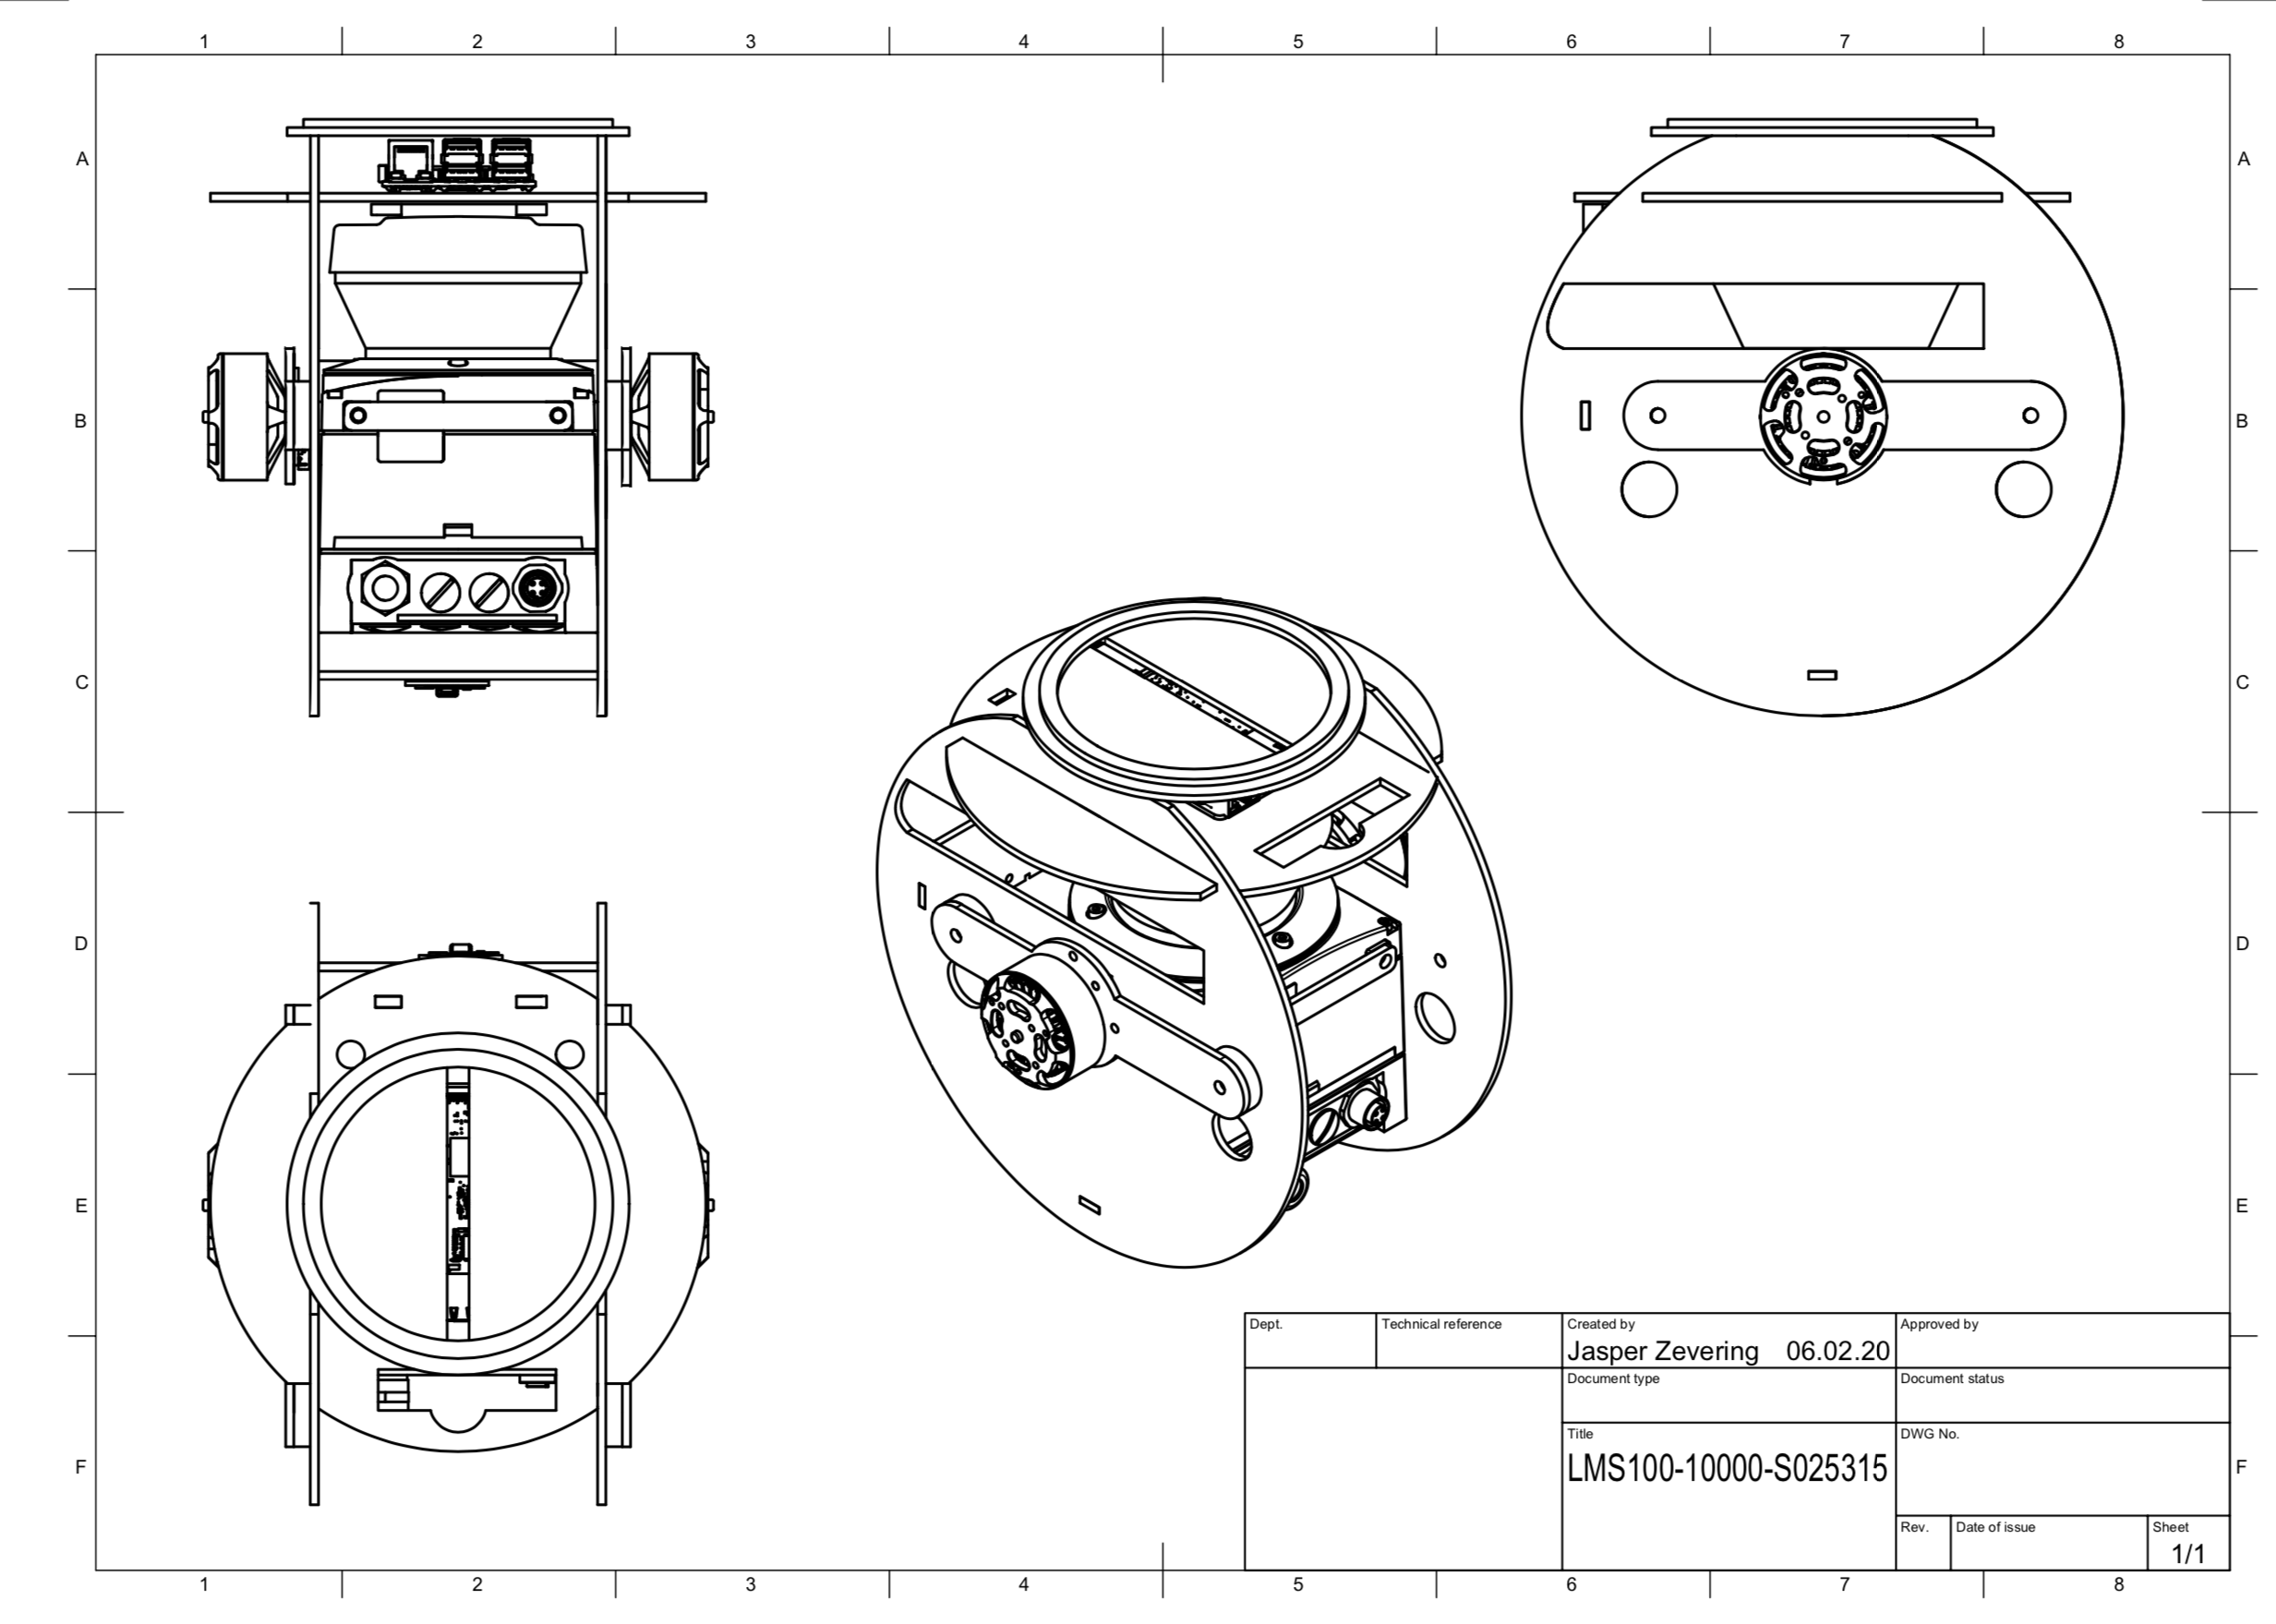
\includegraphics[width=\textwidth]{../Media/BlueprintPNG.png}                                                                                                                                                      
\caption{Blueprint that shows the mechanical structure of the spherical robot.}                                                                                                                                   
\label{sec:TechnicalApproach:fig:blueprint}                                                                                                                                                                       
\end{figure}                                                                                                                                                                                                      
                                                                                                                                                                                                                  
Figure \ref{sec:TechnicalApproach:fig:blueprint} shows a CAD blueprint of the rough interior layout of the mechanical structure of the L.U.N.A sphere, ignoring flywheels and wiring. The blueprint shows that the payload is mounted to supporting structural components which are made of acrylic glass. The raspberry pi model 3 board computer is placed on top of the laser. Above that, another supporting structure can hold additional counterweights to correct for inhomogeneous weight distribution.                                                                                                     
The battery finds its place in front of the laser scanner on another supporting structure. The two brushless motors were each placed on one side of the supporting structure with spacers that leave room for the side IMU underneath one of the motors. Two other IMUs are placed in front of and beneath the laser to ensure coverage of all axes.                                                                                 
                                                                                                                                                                                                                  
\subsection{Sensor Integration}                                                                                                                                                                                   
\label{sec:TechnicalApproach:SensorIntegration}

\begin{figure}                                                                                                                                                                                                    
\centering
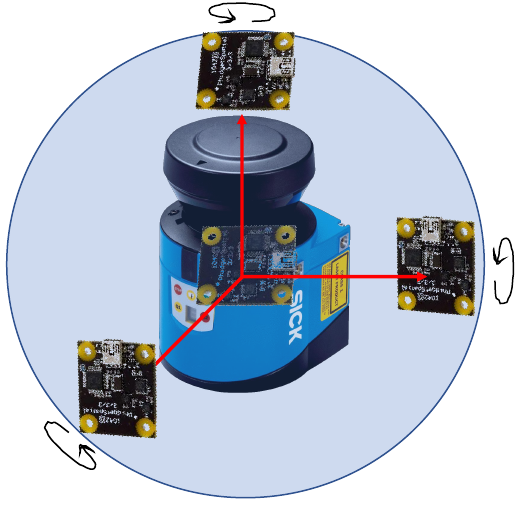
\includegraphics[width=0.5\textwidth]{../Media/virtualIMU.png}                                                                                                                                                      
\caption{Sketch that helps illustrate the combination of 3 IMUs into 1 virtual IMU that simulates being at the center of the sphere.}                                                                                                                           
\label{sec:SensorIntegration:fig:virtual}                                                                                                                                                                       
\end{figure}                                                                                                                                                                                                      

The sensor integration was fully implemented with the Robot Operating System (ROS) using the Ubuntu distribution \href{http://wiki.ros.org/ROSberryPi}{ROSberryPi} which contains a pre-installed ROS version running on a raspberry pi 3.
Overall, three seperate PhidgetsSpacial 10441B IMUs \cite{imuphidgets} were used to keep track of the sphere's pose. Figure \ref{sec:SensorIntegration:fig:virtual} helps illustrate why three IMUs are used instead of just one. Previous prototypes have shown that transforming the data of only one non-centered IMU leads to lower quality measurements. However, combining the measurements of three IMUs, where each of which measures only the static rotation around one of their rotational axes (which also represents a rotation axis of the sphere), leads to better results. Each IMU is perpendicular to the other two, so combining the axis measurements leads to a "virtual" IMU, that simulates being an IMU that takes measurements at the center of the sphere. 

The IMUs also ship with accelerometers that are used to determine the full pose of the sphere. Each IMU calculates their pose separately, using a quaternion extended Kalman filter (QEKF). However, combining those poses into one did not have any positive effect, but only made the software more resource demanding and slow. Thus only the pose of the bottom IMU's accelerometers are used to keep track of the pose.

The motors are controlled using the piGPIO library. The GPIO signals are forwarded by the pins to two ESCs that drive the motors. 

Unfortunately, the brass weights were not drilled in the very center, causing an imbalance when rotating. The resulting vibrations inhibit the movement of the sphere thus a controller was implemented that measures the extent of the vibrations using standard deviations of the IMU's axes that are not rolled over and adjusts the throttle of the motors accordingly. This was done with a simple two-point controller with hysteresis which already leads to satisfying results. Considering the translational velocity of the sphere in a controller is not possible, because the speed of the sphere is calculated by the rotational speed and therefore slippage of the sphere would break such a controller. 

\subsection{Point Cloud Processing}                                                                                                                                                                                  
\label{sec:TechnicalApproach:3dMapping}
For the processing of the point cloud the 3D Toolkit (3DTK) was used. This provides multiple methods and algorithms for processing 3D point clouds, especially the 6D Simultaneous Localization And Mapping (SLAM) algorithm (see \cite{JFR2006}). To lower the stress of the largely exhausted microcontroller, the processing of raw data was outsourced to a server-like operating pc. Therefore only the time-stamped raw data of the IMUs and laser-scanner had to be transferred and the estimation of the pose and the SLAM algorithm itself are performed external of the sphere. For this prototype the transfer was realized by using the Host-function of ROS, giving the external pc the possibility to subscribe to the topics and process them. 3DTK itself takes pairs of files, one representing the pose, one the laser scanner data, and each file named by the time-stamp with an identifier if it is scan-data or pose. With a more potent micro controller this could be performed directly onboard. Also, the use of USB-connected IMUs and ROS as transfer-mechanism of data leaves much potential for enhancement and therefore relieving the internal controller.
